\documentclass[12pt,english,pdftex,a4paper]{book}

%%%%%%%%%%%%%%%%%%%%%%%%%%%%%%%%%%%%%%%%%%%%%%%%%%%%%%%%%%%%%%%%%%%%%%%%%%%%%
% Parameters
%%%%%%%%%%%%%%%%%%%%%%%%%%%%%%%%%%%%%%%%%%%%%%%%%%%%%%%%%%%%%%%%%%%%%%%%%%%%%

%%%%%%%%%%%%%%%%%%%%%%%%%%%%%%%%%%%%%%%%%%%%%%%%%%%%%%%%%%%%%%%%%%%%%%%%%%%%%
% parameters.tex
%%%%%%%%%%%%%%%%%%%%%%%%%%%%%%%%%%%%%%%%%%%%%%%%%%%%%%%%%%%%%%%%%%%%%%%%%%%%%

\newcommand{\licTitle}{Licentitate Thesis Template}
\newcommand{\licAuthor}{Author's Name}
\newcommand{\licYear}{2017}

\newif\ifShowHalfPage
\newif\ifShowLayout
\newif\ifShowGrid
\newif\ifSpaper
\newif\ifSclip
\newif\ifIncludePDFs

%%%%%%%%%%%%%%%%%%%%%%%%%%%%%%%%%%%%%%%%%%%%%%%%%%%%%%%%%%%%%%%%%%%%%%%%%%%%%

% \IncludePDFstrue      % Turn this on to include PDFs of the papers
  \Spapertrue           % Enable S5 format
  \Scliptrue            % Clip to S5 format (assuming S5 is enabled)
  \ShowHalfPagetrue     % Show half-page
% \ShowLayouttrue       % Show layout info at the end
% \ShowGridtrue         % Show mm grid at each peage
      % Here comes important parameters

%%%%%%%%%%%%%%%%%%%%%%%%%%%%%%%%%%%%%%%%%%%%%%%%%%%%%%%%%%%%%%%%%%%%%%%%%%%%%
% Specify the used packages
%%%%%%%%%%%%%%%%%%%%%%%%%%%%%%%%%%%%%%%%%%%%%%%%%%%%%%%%%%%%%%%%%%%%%%%%%%%%%

%%%%%%%%%%%%%%%%%%%%%%%%%%%%%%%%%%%%%%%%%%%%%%%%%%%%%%%%%%%%%%%%%%%%%%%%%%%%%
% preamble.tex
%%%%%%%%%%%%%%%%%%%%%%%%%%%%%%%%%%%%%%%%%%%%%%%%%%%%%%%%%%%%%%%%%%%%%%%%%%%%%

\usepackage{lmodern}
\renewcommand{\sfdefault}{lmss}
\renewcommand{\ttdefault}{lmtt}

\usepackage[T1]{fontenc}
\usepackage[latin9]{inputenc}

\usepackage{geometry}
\geometry{verbose,tmargin=40mm,bmargin=46mm,lmargin=38mm,rmargin=32mm}

\setcounter{secnumdepth}{3}
\setcounter{tocdepth}{1}

\usepackage{color}
\usepackage{babel}
\usepackage{longtable}
\usepackage{float}
\usepackage{mathtools}
\usepackage{enumitem}
\usepackage{amsmath}
\usepackage{amsthm}
\usepackage{amssymb}
\usepackage{mathdots}
\usepackage{stmaryrd}

%%%%%%%%%%%%%%%%%%%%%%%%%%%%%%%%%%%%%%%%%%%%%%%%%%%%%%%%%%%%%%%%%%%%%%%%%%%%%

\usepackage[unicode=true]{hyperref}

\hypersetup{
  pdftitle           = {\licTitle},
  pdfauthor          = {\licAuthor},
  pdfsubject         = {Licentiate Thesis in Theoretical Physics},
  bookmarks          = true,
  bookmarksnumbered  = true,
  bookmarksopen      = true,
  bookmarksopenlevel = 1,
  breaklinks         = true,
  pdfborder          = {0 0 0},
  pdfborderstyle     = {},
  backref            = false,
  colorlinks         = true,
  linkcolor          = blue,
  urlcolor           = blue,
  citecolor          = blue,
  anchorcolor        = green,
  pdfstartview       = {Fit},
  pdfpagelayout      = {TwoPageRight},
  linktocpage, pagebackref, hyperfigures
}

\ifSpaper
  \hypersetup{colorlinks=false}
\fi

%%%%%%%%%%%%%%%%%%%%%%%%%%%%%%%%%%%%%%%%%%%%%%%%%%%%%%%%%%%%%%%%%%%%%%%%%%%%%

% S5 papersize = { 165mm, 242mm } * 12 / 10.95 + { 6mm, 0mm }

\ifSpaper
  \geometry{
    verbose,
    papersize = { 184.82mm, 265.2mm }, 
    tmargin   = 27.1mm,
    bmargin   = 27.1mm,
    lmargin   = 22.41mm,
    rmargin   = 22.41mm,
    marginparwidth = 20mm
  }
\fi

%%%%%%%%%%%%%%%%%%%%%%%%%%%%%%%%%%%%%%%%%%%%%%%%%%%%%%%%%%%%%%%%%%%%%%%%%%%%%

% Optionally show the diagram of the page layout

\ifShowLayout
  \usepackage[noframe]{showframe} 
  \usepackage{layouts}
  \makeatletter
  \let\FontSize=\f@size
  \makeatother
\fi

%%%%%%%%%%%%%%%%%%%%%%%%%%%%%%%%%%%%%%%%%%%%%%%%%%%%%%%%%%%%%%%%%%%%%%%%%%%%%

% Use sanserif for headings

\usepackage[{sf,bf}]{titlesec}

%%%%%%%%%%%%%%%%%%%%%%%%%%%%%%%%%%%%%%%%%%%%%%%%%%%%%%%%%%%%%%%%%%%%%%%%%%%%%

% \usepackage[margin=10pt,font=small,labelfont=bf]{caption} 
\usepackage[margin=10pt,labelfont=bf]{caption} 

% Turn off nasty worning for overfull and underfull hboxes
% \hbadness=10000
% \hfuzz=50pt

%%%%%%%%%%%%%%%%%%%%%%%%%%%%%%%%%%%%%%%%%%%%%%%%%%%%%%%%%%%%%%%%%%%%%%%%%%%%%

\usepackage{cite} % Compressed citations

%%%%%%%%%%%%%%%%%%%%%%%%%%%%%%%%%%%%%%%%%%%%%%%%%%%%%%%%%%%%%%%%%%%%%%%%%%%%%

\pdfmapfile{+rsfso.map}  % More upright mathscr
\DeclareSymbolFont{rsfso}{U}{rsfso}{m}{n}
\DeclareSymbolFontAlphabet{\mathscr}{rsfso}

% \usepackage[scaled=1.1]{rsfso}   % Turn also mathcal into rfso

%%%%%%%%%%%%%%%%%%%%%%%%%%%%%%%%%%%%%%%%%%%%%%%%%%%%%%%%%%%%%%%%%%%%%%%%%%%%%

%\usepackage{etoolbox} % a toolbox of programming tools

\usepackage{xfrac}  % Split-level fractions (\sfrac)

%%%%%%%%%%%%%%%%%%%%%%%%%%%%%%%%%%%%%%%%%%%%%%%%%%%%%%%%%%%%%%%%%%%%%%%%%%%%%

%\usepackage{graphicx}
%\DeclareGraphicsExtensions{.png, .jpg, .jpeg, .pdf} %GIF doesn't work
%\pdfcompresslevel=9
%\graphicspath{{figures/}}

%%%%%%%%%%%%%%%%%%%%%%%%%%%%%%%%%%%%%%%%%%%%%%%%%%%%%%%%%%%%%%%%%%%%%%%%%%%%%

\usepackage{tensind} 
\tensordelimiter{?}

%%%%%%%%%%%%%%%%%%%%%%%%%%%%%%%%%%%%%%%%%%%%%%%%%%%%%%%%%%%%%%%%%%%%%%%%%%%%%

\usepackage{xcolor}
\usepackage{colortbl}

\let\myHlineC\hline

\newcommand{\bHlineC}{
  \renewcommand{\hline}{\arrayrulecolor{lightgray}\myHlineC\arrayrulecolor{black}}
  \newcolumntype{|}{!{\color{lightgray}\vline}}
}

\newcommand{\eHlineC}{
  \renewcommand{\hline}{\myHlineC}
  \newcolumntype{|}{!{\color{black}\vline}}
}

%%%%%%%%%%%%%%%%%%%%%%%%%%%%%%%%%%%%%%%%%%%%%%%%%%%%%%%%%%%%%%%%%%%%%%%%%%%%%

\newcommand{\bSe}{\begin{subequations}} 
\newcommand{\eSe}{\end{subequations}}

\newcommand{\bWe}{\begin{widetext}} 
\newcommand{\eWe}{\end{widetext}}

%%%%%%%%%%%%%%%%%%%%%%%%%%%%%%%%%%%%%%%%%%%%%%%%%%%%%%%%%%%%%%%%%%%%%%%%%%%%%

\allowdisplaybreaks

%%%%%%%%%%%%%%%%%%%%%%%%%%%%%%%%%%%%%%%%%%%%%%%%%%%%%%%%%%%%%%%%%%%%%%%%%%%%%

% Remove if we do not have tikz

\usepackage{tikz,amsmath,amssymb,bm,color,cancel}
\usetikzlibrary{shapes,arrows}
\usetikzlibrary{calc}
\usetikzlibrary{positioning}
\usetikzlibrary{decorations.pathreplacing}

%%%%%%%%%%%%%%%%%%%%%%%%%%%%%%%%%%%%%%%%%%%%%%%%%%%%%%%%%%%%%%%%%%%%%%%%%%%%%

\usepackage{lastpage}

%%%%%%%%%%%%%%%%%%%%%%%%%%%%%%%%%%%%%%%%%%%%%%%%%%%%%%%%%%%%%%%%%%%%%%%%%%%%%

% Load fancyhdr after specifying the geometry (bogus if loaded before)
\usepackage{fancyhdr}
\usepackage[iso]{datetime}

\fancypagestyle{empty}
{
    \fancyhf{} % clear all header and footer fields
}

\fancypagestyle{plain}
{
    \fancyhf{} % clear all header and footer fields
    \fancyfoot[LE,RO]{\thepage}
    \fancyfoot[RE,LO]{}
    \renewcommand{\headrulewidth}{0pt}
    \renewcommand{\footrulewidth}{0pt}
}

\fancyhf{} % clear all header and footer fields

\fancyhead[LE,RO]{\thepage}
\fancyhead[RE]{\small\leftmark}
\fancyhead[LO]{\small\rightmark}
\fancyhead[CE]{}

\renewcommand{\headrulewidth}{0pt}
\renewcommand{\footrulewidth}{0pt}

%%%%%%%%%%%%%%%%%%%%%%%%%%%%%%%%%%%%%%%%%%%%%%%%%%%%%%%%%%%%%%%%%%%%%%%%%%%%%

\pagestyle{fancy}

% Don't convert marks to upperase

% printindex sets the pagestyle to plain, to counter this, we can redefine this pagestyle. 
% If we use the fancy pagestyle throughout our document add the following to the preamble:
%\renewcommand{\ps@plain}{\pagestyle{fancy}}

\frontmatter

%%%%%%%%%%%%%%%%%%%%%%%%%%%%%%%%%%%%%%%%%%%%%%%%%%%%%%%%%%%%%%%%%%%%%%%%%%%%%

\usepackage[titletoc]{appendix}

\usepackage[nottoc,notlof,notlot]{tocbibind}

\renewcommand{\sectionmark}[1]{ \markright{\thesection\ #1} }
\renewcommand{\chaptermark}[1]{ \markboth{\chaptername\ \thechapter.\ #1}{\chaptername\ \thechapter.\ #1} }
\renewcommand{\tocetcmark}[1]{ \markboth{#1}{#1} }

% clear empty double pages

%\let\origdoublepage\cleardoublepage
%\newcommand{\clearemptydoublepage}{%
%  \clearpage
%  {\pagestyle{empty}\origdoublepage}%
%}
%\let\cleardoublepage\clearemptydoublepage

\usepackage{emptypage}

%%%%%%%%%%%%%%%%%%%%%%%%%%%%%%%%%%%%%%%%%%%%%%%%%%%%%%%%%%%%%%%%%%%%%%%%%%%%%

\numberwithin{equation}{chapter}
\renewcommand{\theequation}{\thechapter.\arabic{equation}}

\numberwithin{figure}{chapter}
\renewcommand{\thefigure}{\thechapter.\arabic{figure}}

\numberwithin{table}{chapter}
\renewcommand{\thetable}{\thechapter.\arabic{table}}

%%%%%%%%%%%%%%%%%%%%%%%%%%%%%%%%%%%%%%%%%%%%%%%%%%%%%%%%%%%%%%%%%%%%%%%%%%%%%

% \footnotesep is the space between footnotes:
\setlength{\footnotesep}{4mm}

% \footins is the space between the text body and the footnotes:
\setlength{\skip\footins}{6mm}

\selectlanguage{english}

%%%%%%%%%%%%%%%%%%%%%%%%%%%%%%%%%%%%%%%%%%%%%%%%%%%%%%%%%%%%%%%%%%%%%%%%%%%%%

% To include papers:

\usepackage{pdfpages}
\usepackage{ifoddpage}

%%%%%%%%%%%%%%%%%%%%%%%%%%%%%%%%%%%%%%%%%%%%%%%%%%%%%%%%%%%%%%%%%%%%%%%%%%%%%

\usepackage{tabularx}

\newenvironment{pmatrixc}{
  \bgroup\renewcommand{\arraystretch}{1}\begin{pmatrix}
}{
  \end{pmatrix}\egroup
}

\newenvironment{pmatrixr}{
  \bgroup\renewcommand{\arraystretch}{1}\begin{pmatrix*}[r]
}{
  \end{pmatrix*}\egroup
}

%%%%%%%%%%%%%%%%%%%%%%%%%%%%%%%%%%%%%%%%%%%%%%%%%%%%%%%%%%%%%%%%%%%%%%%%%%%%%

\newlength{\InnerEdge}
\newlength{\OuterEdge}
\newcommand{\FrameEdgeColor}{blue!30}
\newcommand{\ShowSubGridColor}{gray!15}
\newcommand{\ShowGridColor}{gray!25}
\newcommand{\ShowGridTextColor}{gray!50}

\ifSpaper
  \setlength{\InnerEdge}{6mm}
\else
  \setlength{\InnerEdge}{8mm}
\fi

\ifSpaper
   \setlength{\OuterEdge}{6mm}
\else
   \setlength{\OuterEdge}{6mm}
\fi

\newcommand{\MarkFrameEdges}{%   
  \begin{tikzpicture}[x=1mm, y=1mm, remember picture, overlay]
      \checkoddpage\ifoddpage
        \draw [dashed,\FrameEdgeColor] 
          ($(current page.south west) + (\InnerEdge,0)$) -- 
          ($(current page.south west) + (\InnerEdge,\paperheight)$);
        \draw [dashed,\FrameEdgeColor] 
          ($(current page.south east) + (-\OuterEdge,0)$) -- 
          ($(current page.south east) + (-\OuterEdge,\paperheight)$);
      \else
        \draw [dashed,\FrameEdgeColor] 
          ($(current page.south east) + (-\InnerEdge,0)$) -- 
          ($(current page.south east) + (-\InnerEdge,\paperheight)$);
        \draw [dashed,\FrameEdgeColor] 
          ($(current page.south west) + (\OuterEdge,0)$) -- 
          ($(current page.south west) + (\OuterEdge,\paperheight)$);
      \fi
  \end{tikzpicture}
}

\newcommand{\ShowGrid}{%   
  \begin{tikzpicture}[x=1mm, y=1mm, remember picture, overlay]
      \checkoddpage\ifoddpage
        \draw[step=1,\ShowSubGridColor,very thin] 
            ($(current page.south west) + (0,0)$) grid 
            ($(current page.south west) + (\paperwidth,\paperheight)$);
        \draw[step=10,\ShowGridColor,very thin] 
            ($(current page.south west) + (0,0)$) grid 
            ($(current page.south west) + (\paperwidth,\paperheight)$);
        \foreach \i in {1,...,30} {
            \node [anchor=west,align=right,\ShowGridTextColor] 
            at ($(current page.south west) + (1,\i * 10)$) {$\i$};
        }
        \foreach \i in {1,...,21} {
            \node [anchor=south,align=center,\ShowGridTextColor] 
            at ($(current page.south west) + (\i * 10,1)$) {$\i$};
        }
        \draw [thin,red] (current page.south west)
           -- ($(current page.south west) + (10,10)$);
      \else
        \draw[step=1,\ShowSubGridColor,very thin] 
            ($(current page.south east) + (0,0)$) grid 
            ($(current page.south east) + (-\paperwidth,\paperheight)$);
        \draw[step=10,\ShowGridColor,very thin] 
            ($(current page.south east) + (0,0)$) grid 
            ($(current page.south east) + (-\paperwidth,\paperheight)$);
        \foreach \i in {1,...,30} {
            \node [anchor=east,align=right,\ShowGridTextColor] 
            at ($(current page.south east) + (-1,\i * 10)$) {$\i$};
        }
        \foreach \i in {1,...,21} {
            \node [anchor=south,align=center,\ShowGridTextColor] 
            at ($(current page.south east) + (-\i * 10,1)$) {$\i$};
        }
        \draw [thin,red] (current page.south east)
           -- ($(current page.south east) + (-10,10)$);
      \fi
  \end{tikzpicture}
}

\ifx\ShowFrameColor\unknown\else
  \renewcommand*\ShowFrameColor{\color{red!10}}
  \AddToShipoutPictureBG{\ShowFramePicture} 
  \ifShowGrid
    \AddToShipoutPictureBG{\ShowGrid}
  \fi
  \AddToShipoutPictureFG{\MarkFrameEdges}
\fi

%%%%%%%%%%%%%%%%%%%%%%%%%%%%%%%%%%%%%%%%%%%%%%%%%%%%%%%%%%%%%%%%%%%%%%%%%%%%%

\makeatletter

\newlength{\TopOffset}
\newlength{\ThumbBoxH}
\newlength{\ThumbBoxW}
\newlength{\ThumbBoxX}
\newlength{\ThumbBoxLargeX}
\newlength{\ThumbBoxY}
\newlength{\OuterMargin}

\newcommand{\ThumbBoxColor}{black!30}

\setlength{\TopOffset}{25.4mm+\hoffset+\topmargin+\headheight+\headsep}
\setlength{\ThumbBoxH}{23mm}
\setlength{\ThumbBoxW}{70mm}
\setlength{\ThumbBoxX}{14mm}

\ifSpaper
   \setlength{\ThumbBoxLargeX}{30mm}
\else
   \setlength{\ThumbBoxLargeX}{24mm}
\fi

\setlength{\ThumbBoxY}{\TopOffset-\ThumbBoxH/2}

\setlength{\OuterMargin}{25.4mm+\hoffset+\evensidemargin}

\newcommand{\ThumbBox}[2]{%
  \begin{tikzpicture}[x=1mm, y=1mm, remember picture, overlay]
      \checkoddpage\ifoddpage
        \node [anchor=north,rotate=90,draw,rectangle, very thin, rounded corners=5pt,
          color=\ThumbBoxColor,fill=\ThumbBoxColor,minimum width=\ThumbBoxH,minimum height=\ThumbBoxW] 
          at ($(current page.north east) - (\ThumbBoxX,\ThumbBoxY+\value{chapter}*\ThumbBoxH+#2*\ThumbBoxH)$) 
          {};
        \node [anchor=north,rotate=90,text width=\ThumbBoxH,align=flush center,font=\sffamily] 
          at ($(current page.north east) - (\ThumbBoxX-1,\ThumbBoxY+\value{chapter}*\ThumbBoxH+#2*\ThumbBoxH)$) 
          {\color{white}\textbf{#1}};
      \else
        \node [anchor=south,rotate=90,draw,rectangle, very thin, rounded corners=5pt,
          color=\ThumbBoxColor,fill=\ThumbBoxColor,minimum width=\ThumbBoxH,minimum height=\ThumbBoxW] 
          at ($(current page.north west) - (-\ThumbBoxX,\ThumbBoxY+\value{chapter}*\ThumbBoxH+#2*\ThumbBoxH)$) 
          {};
        \node [anchor=south,rotate=90,text width=\ThumbBoxH,align=flush center,font=\sffamily] 
          at ($(current page.north west) - (-\ThumbBoxX+1,\ThumbBoxY+\value{chapter}*\ThumbBoxH+#2*\ThumbBoxH)$) 
          {\color{white}\textbf{#1}};
      \fi
  \end{tikzpicture}
}

\newcommand{\ThumbBoxLarge}[2]{%
  \checkoddpage\ifoddpage
    \begin{tikzpicture}[x=1mm, y=1mm, remember picture, overlay]
      \node [anchor = west,
        draw, rectangle, very thin, rounded corners=5pt, inner sep = 5,
        fill = \ThumbBoxColor, color = \ThumbBoxColor,
        minimum height = \ThumbBoxH, minimum width = \ThumbBoxW, text width = \ThumbBoxW,
        align = flush left, font = \sffamily] 
        at ($(current page.north east) - (\OuterMargin+\ThumbBoxLargeX,\ThumbBoxY+\value{chapter}*\ThumbBoxH+#2*\ThumbBoxH)$)
        {\color{white}\fontsize{23pt}{0em}\selectfont\textbf{~~#1}};
    \end{tikzpicture}
  \fi
}

\newcommand{\labelPaper}[1]{%
   \let\orglabel\label
   \let\label\@gobble
   \edef\@currentlabel{#1\unskip}%
   \let\label\orglabel
}

\newcommand{\overlayPaperInfo}[1]{%
  \begin{tikzpicture}[x=1mm, y=1mm, remember picture, overlay]
    \node [anchor=south east,align=flush left,text width=\textwidth, inner sep = 0] 
      at ($(current page.north east) - (\OuterMargin,\TopOffset+\textheight)$) {#1};
  \end{tikzpicture}
}

\newcounter{PaperSubFolio}
\newcommand{\PaperSubFolioFontSize}{12}

\ifShowLayout
  \tikzset{folioFill/.style={red!10}}
\else
  \tikzset{folioFill/.style={white,fill=white}}
\fi

\newcommand{\overlayPaperFolio}[3]{%
  \begin{tikzpicture}[x=1mm, y=1mm, remember picture, overlay]
      \checkoddpage\ifoddpage
        \node [anchor=south,draw,rectangle,folioFill] 
          at ($(current page.south) + (#2,#3)$)
          {\fontsize{\PaperSubFolioFontSize}{0}\selectfont\color{black}
          \textsc{Paper \PaperID}~--~\thePaperSubFolio~\color{black!60}(\thepage)};
      \else
        \node [anchor=south,draw,rectangle,folioFill] 
          at ($(current page.south) + (-#2,#3)$)
          {\fontsize{\PaperSubFolioFontSize}{0}\selectfont\color{black}
          \textsc{Paper \PaperID}~--~\thePaperSubFolio~\color{black!60}(\thepage)};
      \fi
  \end{tikzpicture}
  \stepcounter{PaperSubFolio}
}

\makeatother

%%%%%%%%%%%%%%%%%%%%%%%%%%%%%%%%%%%%%%%%%%%%%%%%%%%%%%%%%%%%%%%%%%%%%%%%%%%%%

\makeatletter
\newcommand{\lofwithouttitle}{\@starttoc{lof}}
\newcommand{\lotwithouttitle}{\@starttoc{lot}}
\newcommand{\tocwithouttitle}{\@starttoc{toc}}
\makeatother

%%%%%%%%%%%%%%%%%%%%%%%%%%%%%%%%%%%%%%%%%%%%%%%%%%%%%%%%%%%%%%%%%%%%%%%%%%%%%

\usepackage{tocloft}

\cftpagenumbersoff{part}

\renewcommand{\cftpartfont}{\scshape\normalsize}
\renewcommand{\cftpartpagefont}{\bfseries\rmfamily\normalsize}
\renewcommand{\cftbeforepartskip}{6mm}
\renewcommand{\cftpartafterpnum}{\vspace{2mm}}

\renewcommand{\cftchapfont}{\rmfamily\normalsize}
\renewcommand{\cftchappagefont}{\rmfamily\normalsize}
\renewcommand{\cftchapleader}{\cftdotfill{\cftchapdotsep}}
\renewcommand{\cftchapdotsep}{\cftdotsep}
\setlength{\cftchapindent}{8mm}
\setlength{\cftbeforechapskip}{1mm}

\renewcommand{\cftsecfont}{\rmfamily\normalsize}
\renewcommand{\cftsecpagefont}{\rmfamily\normalsize}
\setlength{\cftsecindent}{14mm}

\setlength{\cftsubsecindent}{19mm}
\setlength{\cftsubsubsecindent}{26mm}

\setlength{\cftbeforefigskip}{\cftbeforechapskip}
\setlength{\cftbeforetabskip}{\cftbeforechapskip}

%%%%%%%%%%%%%%%%%%%%%%%%%%%%%%%%%%%%%%%%%%%%%%%%%%%%%%%%%%%%%%%%%%%%%%%%%%%%%
        % Premable with the used packages

%%%%%%%%%%%%%%%%%%%%%%%%%%%%%%%%%%%%%%%%%%%%%%%%%%%%%%%%%%%%%%%%%%%%%%%%%%%%%
% Useful definitions
%%%%%%%%%%%%%%%%%%%%%%%%%%%%%%%%%%%%%%%%%%%%%%%%%%%%%%%%%%%%%%%%%%%%%%%%%%%%%

% Math upright symbols (see ISO 80000 and NIST SP 811)

\global\long\def\dd{\mathrm{d}}
\global\long\def\ee{\mathrm{e}}
\global\long\def\ii{\mathrm{i}}

\global\long\def\tr{\mathsf{{\scriptscriptstyle T}}}

\global\long\def\diag{\operatorname{diag}}
\global\long\def\Tr{\operatorname{Tr}}

% Tensors; e.g., \tudu = tensor with up-down-up indices

\global\long\def\tudu#1#2#3#4{?{\mbox{\ensuremath{#1}}}^{#2}{}_{#3}{}^{#4}?}
\global\long\def\tdud#1#2#3#4{?{\mbox{\ensuremath{#1}}}{}_{#2}{}^{#3}{}_{#4}?}
\global\long\def\tud#1#2#3{?{\mbox{\ensuremath{#1}}}^{#2}{}_{#3}?}
\global\long\def\tdu#1#2#3{?{\mbox{\ensuremath{#1}}}{}_{#2}{}^{#3}?}
\global\long\def\tuu#1#2#3{?{\mbox{\ensuremath{#1}}}{}^{#2}{}^{#3}?}
\global\long\def\tdd#1#2#3{?{\mbox{\ensuremath{#1}}}{}_{#2}{}_{#3}?}

% Lie derivative
\global\long\def\Lie{\mathrm{\pounds}}

%%%%%%%%%%%%%%%%%%%%%%%%%%%%%%%%%%%%%%%%%%%%%%%%%%%%%%%%%%%%%%%%%%%%%%%%%%%%%

\begin{document}

%%%%%%%%%%%%%%%%%%%%%%%%%%%%%%%%%%%%%%%%%%%%%%%%%%%%%%%%%%%%%%%%%%%%%%%%%%%%%
% Thesis OUTLINE
%%%%%%%%%%%%%%%%%%%%%%%%%%%%%%%%%%%%%%%%%%%%%%%%%%%%%%%%%%%%%%%%%%%%%%%%%%%%%

% The outline of the thesis that is a comprehensive summary of papers:
% (optional items are given italic)
% ============================================= Front matter
% - Title page, recto
% - Printing info (abstract), verso
% - Dedication page, recto
% - List of papers, recto
% - Table of Contents , recto
% - List of Figures/Tables, recto
% - Preface (and/or/including author's contribution, acknowledgments), recto
% - Abbreviations, recto
% ============================================= Text
% Part I. Comprehensive summary
% - Chapter 1. Introduction
% - Chapter 2, . . .
% - Summary
% - Svensk sammanfattning 
% (A short summary in Swedish should be be included if the thesis 
% is written in a foreign language.)
% ============================================= Back matter
% - References
% ============================================= Appendix
% Part II. Papers
% - Paper 1, . . .
% ============================================= Typography, A4
% Paper: 210 x 297 (A4)
% Text: 140 x 211
% Font: 12pt
% Inner offset: 8
% Margins: 
% T = 40, B = 46, T+B = 96
% I = 38, O = 32, I+O = 70
% ============================================= Typography, S5
% Paper: 165 x 242 (S5)
% Text: 140 x 211
% Font: 11pt
% Margins: 
% T = 17.5, B = 17.5, T+B = 35
% I = 22.5, O = 22.5, I+O = 45

\frontmatter

%----------------------------------------------------------------------------
% TITLE PAGE
%----------------------------------------------------------------------------

\pagestyle{empty}
\thispagestyle{empty}

\ifShowHalfPage
  \pagenumbering{arabic}  % Set folio: F1, F2, ...
  \renewcommand*{\thepage}{F\arabic{page}}
  \ifSpaper
    
\includepdf[pages = {-}, scale = 0.93, offset = -5mm 1.5mm]
      {cover/half-page.pdf}
  \else
    % dimensions = 174 x 246 scaled 0.828 = 144 x 204
    
\includepdf[pages = {-}, scale = 0.828, offset = -2mm 4mm]
      {cover/half-page.pdf}
  \fi
  \cleardoublepage
  \pagenumbering{roman}  % Set folio: i, ii, ...
\fi

\ifSpaper
  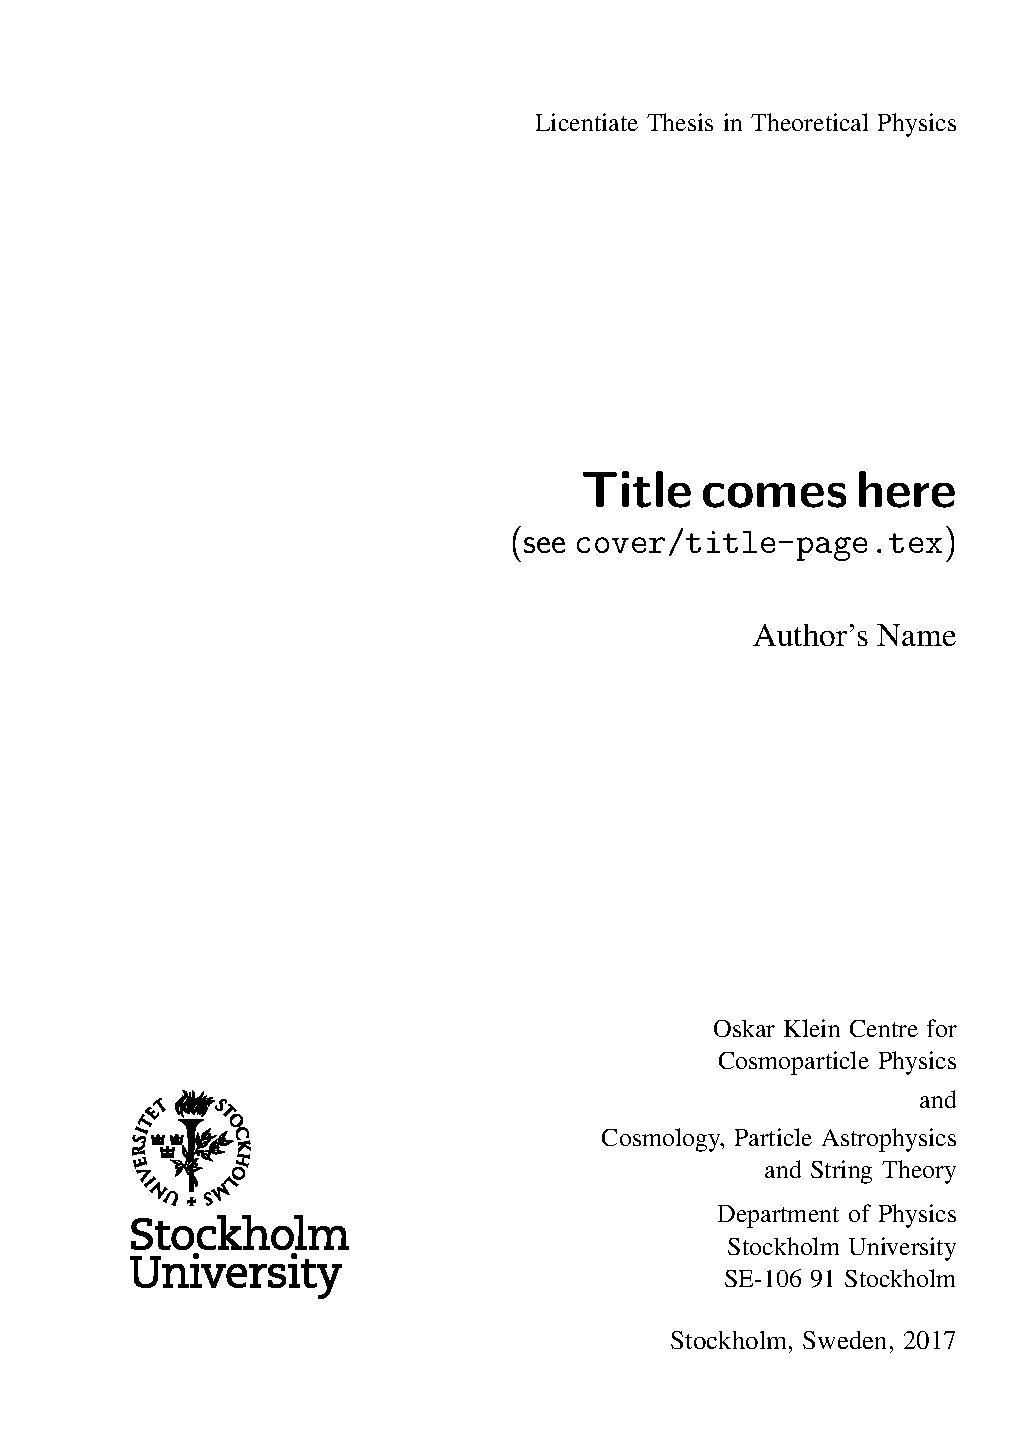
\includepdf[pages = {-}, scale = 0.93, offset = -5mm 1.5mm]
    {cover/title-page.pdf}
\else
  % dimensions = 174 x 246 scaled 0.828 = 144 x 204
  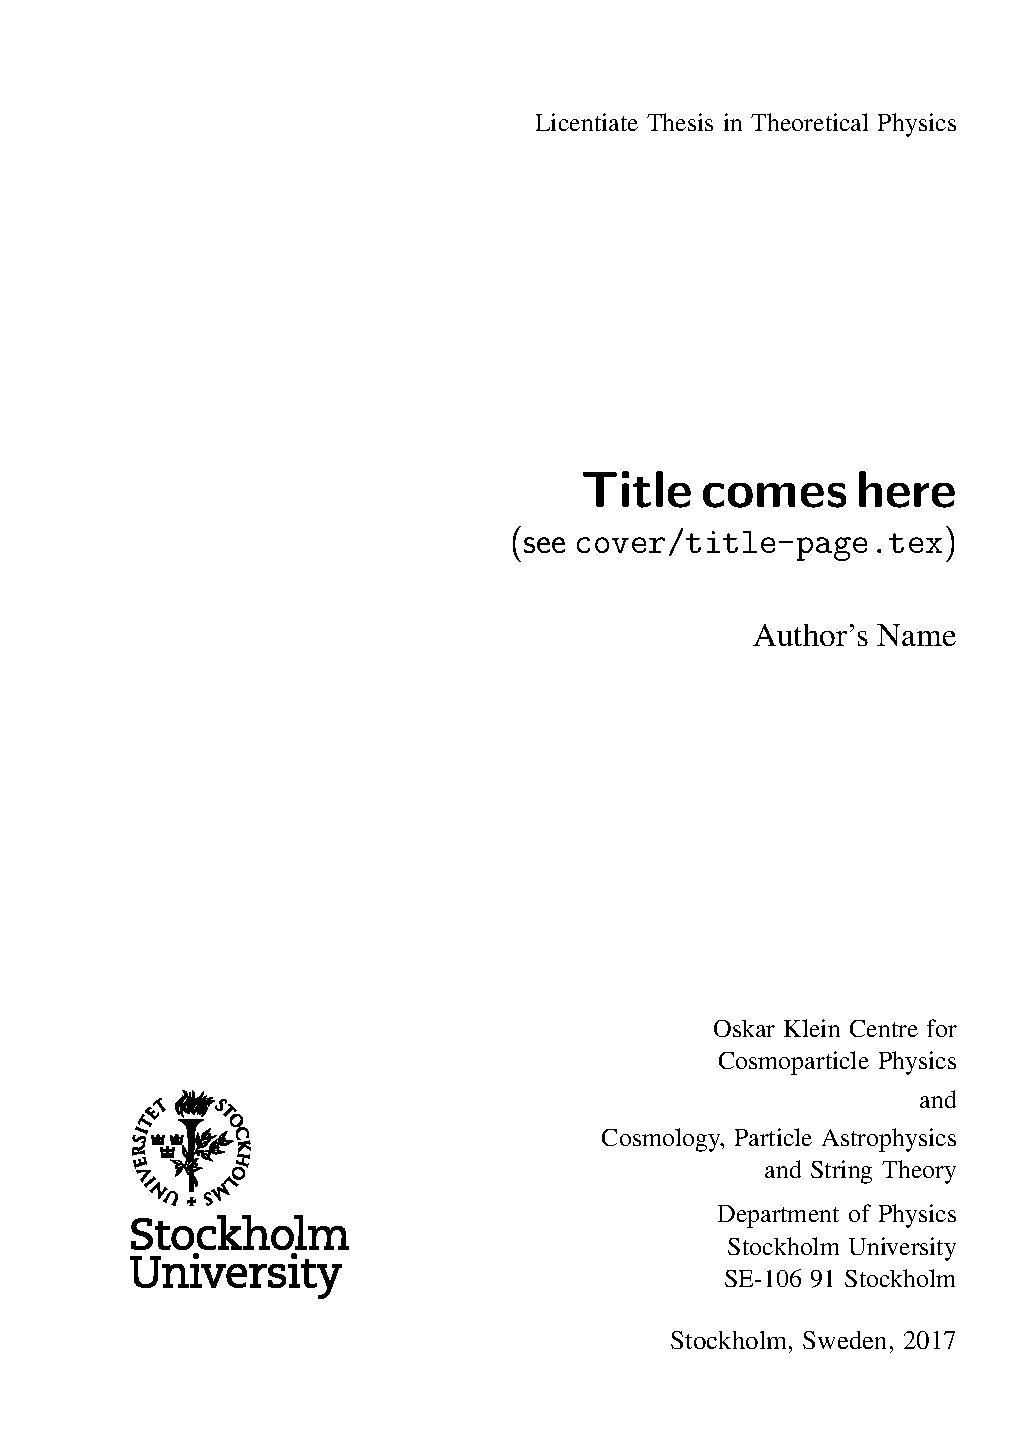
\includepdf[pages = {-}, scale = 0.828, offset = -2mm 4mm]
    {cover/title-page.pdf}
\fi

%----------------------------------------------------------------------------
% PRINTING INFO
%----------------------------------------------------------------------------

% The printing info is on the title page verso.
\clearpage
~\vspace{183mm}

% The abstract of the thesis will be printed on the spikblad 
% which will be generated upon the electronic spikning. 
% However, if the author believes it necessary to also include 
% the abstract in the printed document this is were it should go.

\noindent
  Printed: 2017-10-23\\[5mm]
  pp. i--\pageref*{lastPageOfFrontMatter},
     1--\pageref*{lastPageOfPartI},
     \copyright~2017 by \licAuthor\\[1mm]
  Typeset in pdf\LaTeX

\cleardoublepage

%----------------------------------------------------------------------------
% List of Papers
%----------------------------------------------------------------------------

\fancypagestyle{plain}
{
    \fancyhf{}
    \fancyfoot[LE,RO]{\thepage}
    \fancyfoot[RE,LO]{}
    \renewcommand{\headrulewidth}{0pt}
    \renewcommand{\footrulewidth}{0pt}
}

\fancyhf{}
\fancyhead[LE,RO]{\thepage}
\fancyhead[RE]{\sc\leftmark}
\fancyhead[LO]{\sc\rightmark}


\chapter*{List of Papers}

\noindent The following papers are included in the thesis. They are
referred to by their Roman numerals in the text.

\begin{description}[labelindent=2mm,labelwidth=10mm,leftmargin=12mm,labelsep=0mm]

\item [{\ref{art:A}}] 
Authors,
\emph{Title},
{[}\href{https://arxiv.org/abs/1706.07806}{1706.07806}{]}

\item [{\ref{art:B}}]
Authors,
\emph{Title},
{[}\href{https://arxiv.org/abs/1708.07833}{1708.07833}{]}

\item [{\ref{art:C}}] 
Authors,
\emph{Title},
{[}\href{https://arxiv.org/abs/1703.07787}{1703.07787}{]}

\end{description}
\vspace{2ex}

\noindent The following papers are complementary and not included
in the thesis. They are quoted as ordinary references in the main
text.

\begin{description}[labelindent=2mm,labelwidth=10mm,leftmargin=12mm,labelsep=0mm]

\item [{IV}]
Authors 
\emph{Title}, 
{[}\href{https://arxiv.org/abs/1706.00787}{1706.00787}{]}

\item [{V}]
Authors,
\emph{Title},
{[}\href{https://arxiv.org/abs/1710.06434}{1710.06434}{]}

\item [{VI}] 
Authors,
\emph{Title},
{[}\href{https://arxiv.org/abs/1409.1909}{1409.1909}{]}

\end{description}
\vspace{2ex}

\noindent The chronological order of the papers is ...


%----------------------------------------------------------------------------
% CONTENTS
%----------------------------------------------------------------------------

\cleardoublepage

\pdfbookmark[1]{Table of Contents}{indexname}
\chapter*{Contents}
\markboth{Contents}{Contents}
\tocwithouttitle

\chapter*{Illustrations}
\markboth{Illustrations}{Illustrations}
\addcontentsline{toc}{chapter}{Illustrations}
\vspace{0.2em}

\subsection*{List of Figures}\vspace{-0.5em}
\lofwithouttitle\vspace{0.2em}

\subsection*{List of Tables}\vspace{-0.5em}
\lotwithouttitle

\cleardoublepage

%%%%%%%%%%%%%%%%%%%%%%%%%%%%%%%%%%%%%%%%%%%%%%%%%%%%%%%%%%%%%%%%%%%%%%%%%%%%%
% front-matter/preface.tex
%%%%%%%%%%%%%%%%%%%%%%%%%%%%%%%%%%%%%%%%%%%%%%%%%%%%%%%%%%%%%%%%%%%%%%%%%%%%%

\chapter*{Preface}

\addcontentsline{toc}{chapter}{Preface}
\markboth{Preface}{Preface}

This licentiate thesis is a thesis by publication consisting of two
major parts:  introductory chapters comprising a summary of the
scientific results, and  the corresponding papers published or submitted
for publication.

. . .

\clearpage~\vspace{14mm}

\section*{Contribution to papers}
\vspace{5mm}

\begin{description}
  
\item [{Paper~I.}] 
contributions...

\item [{Paper~II.}] 
contributions...

\item [{Paper~III.}] 
contributions...

\item [{Paper~IV.}] 
contributions...

\item [{Paper~V.}] 
contributions...

\item [{Paper~VI.}] 
contributions...
\end{description}

\clearpage~\vspace{14mm}

\section*{Acknowledgments}

\vspace{5mm}

My deepest gratitude goes to ...



\vspace{5mm}
\noindent \begin{flushright}
\licAuthor\\
Stockholm, \today
\par\end{flushright}

%%%%%%%%%%%%%%%%%%%%%%%%%%%%%%%%%%%%%%%%%%%%%%%%%%%%%%%%%%%%%%%%%%%%%%%%%%%%%
% front-matter/notation.tex
%%%%%%%%%%%%%%%%%%%%%%%%%%%%%%%%%%%%%%%%%%%%%%%%%%%%%%%%%%%%%%%%%%%%%%%%%%%%%

\chapter*{Abbreviations}

\addcontentsline{toc}{chapter}{Abbreviations and notation}
\markboth{}{}

\noindent \bgroup\def\arraystretch{1.2}%
\begin{longtable}[l]{ll}
  
AdS & anti-de Sitter \cite{Misner:1974qy}\tabularnewline
. & .\tabularnewline
. & .\tabularnewline
. & .\tabularnewline
SM & The Standard Model of particle physics\tabularnewline

\end{longtable}\egroup


%%%%%%%%%%%%%%%%%%%%%%%%%%%%%%%%%%%%%%%%%%%%%%%%%%%%%%%%%%%%%%%%%%%%%%%%%%%%%
% MAIN MATTER
%%%%%%%%%%%%%%%%%%%%%%%%%%%%%%%%%%%%%%%%%%%%%%%%%%%%%%%%%%%%%%%%%%%%%%%%%%%%%

\label{lastPageOfFrontMatter}
\cleardoublepage

\renewcommand{\thepage}{\roman{page}}
\setcounter{page}{1}

\renewcommand{\thechapter}{\arabic{chapter}}
\setcounter{chapter}{0}

\mainmatter

\pagestyle{fancy}

\newcommand{\ChapterThumb}{\ThumbBox{Chapter \arabic{chapter}}{0}}

\fancypagestyle{plain}
{
    \fancyhf{}
    \fancyfoot[LE,RO]{\thepage}
    \fancyfoot[RE,LO]{\small\textcolor{black!35}{
        \ifSpaper\else ~\\[-1ex] \fi
        \textcolor{black!20}{\rule{75mm}{0.4pt}}~\\
        \licAuthor,
        \emph{\licTitle},
        SU \licYear
        }
    }
    \renewcommand{\headrulewidth}{0pt}
    \renewcommand{\footrulewidth}{0pt}
    \fancyhead[CE]{\ChapterThumb}
    \fancyhead[CO]{\ChapterThumb}
}

\fancyhf{}
\fancyhead[LE,RO]{\thepage}
\fancyhead[RE]{\small\leftmark}
\fancyhead[LO]{\small\rightmark}
\fancyhead[CE]{\ChapterThumb}
\fancyhead[CO]{\ChapterThumb}

\phantomsection
\addcontentsline{toc}{part}{Part I \;Comprehensive Summary}

%----------------------------------------------------------------------------
% MAIN TEXT
%----------------------------------------------------------------------------

%%%%%%%%%%%%%%%%%%%%%%%%%%%%%%%%%%%%%%%%%%%%%%%%%%%%%%%%%%%%%%%%%%%%%%%%%%%%%
% chapters/intro.tex
%%%%%%%%%%%%%%%%%%%%%%%%%%%%%%%%%%%%%%%%%%%%%%%%%%%%%%%%%%%%%%%%%%%%%%%%%%%%%

\chapter{Introduction}

The outline of the thesis that is a comprehensive summary of papers 
(optional items are given italic)

\begin{itemize}

  \item Front matter
  \begin{enumerate}
    \item Title page, recto
    \item Printing info (\emph{abstract}), verso
    \item \emph{Dedication page}, recto
    \item List of papers, recto
    \item Table of Contents, recto
    \item \emph{List of Figures/Tables}, recto
    \item \emph{Preface}\\
    (including author's contribution and
    acknowledgments),
    recto
    \item \emph{Abbreviations}, recto
  \end{enumerate}
  
  \item Part I. Comprehensive summary
    \begin{enumerate}
      \item Chapter 1. Introduction
      \item Chapter 2, . . .
      \item Summary
      \item Svensk sammanfattning 
      (A short summary in Swedish should be be included if the thesis is
      written in a foreign language.)
      \item References
    \end{enumerate}
  \item Part II. Papers
    \begin{enumerate}
      \item Paper 1, . . .
      \item Paper 2, . . .
    \end{enumerate}

\end{itemize}

\subsection*{Typography, \textbf{A4}}

\begin{itemize}
\item Paper: 210 mm $\times$ 297 mm
\item Text: 140 mm $\times$ 211 mm
\item Font: 12 pt
\item Inner offset: 8 mm
\item Margins:\\
T = 40, B = 46, T+B = 96\\
I = 38, O = 32, I+O = 70
\end{itemize}

\subsection*{Typography, \textbf{S5}}

\begin{itemize}
\item Paper: 165 mm $\times$ 242 mm
\item Text: 140 mm $\times$ 211 mm
\item Font: 11 pt
\item Margins:\
T = 17.5, B = 17.5, T+B = 35\\
I = 22.5, O = 22.5, I+O = 45
\end{itemize}

\clearpage

\section*{S5 output}

By default, the output is A4 (with 12 pt font). 
To generate S5:

\begin{enumerate}
  \item Uncomment \texttt{\textbackslash{}Spapertrue} flag in 
    \texttt{parameters.tex}.
  \item Compile \texttt{lic-thesis.tex}
  \item Compile \texttt{lic-thesis-S5.tex}
\end{enumerate}

The output \texttt{lic-thesis-S5.pdf} will be in the S5 format.

By enabling \texttt{\textbackslash{}Spapertrue} flag, 
the margins of the master are prepared to be scaled to S5. 
Namely, the master pdf (coming out from \texttt{lic-thesis.tex}) 
is scaled by \texttt{lic-thesis-S5.tex} so the original 
12 pt font will be scaled down to 11 pt in the resulting S5 output.

\paragraph*{Caution:} If you want to continue working with the
A4 output, do not forget to comment \texttt{\textbackslash{}Spapertrue} 
flag in \texttt{parameters.tex}.

\section*{Included PDFs}

You can include PDFs of the included papers by enabling
\texttt{\textbackslash{}IncludePDFstrue} flag in \texttt{parameters.tex}.
By default, the inclusion is disabled (as it slows done the compilation).

The page numbers of the included PDF will be overwritten by
the page numbers of the thesis.
The included papers will be then marked by twofold page numbers. 
For instance,
the folio \texttt{Paper\,II\,\textendash \,5\,(81)} marks a page
from Paper II having the internal (article) page number 5 and the
overall (thesis) page number 81.
To modify the position of the page numbers, see the arguments 
\texttt{\#5} and \texttt{\#6} in \texttt{\textbackslash{}paperSection}.
To debug the positions, you can temporarily enable the flags
\texttt{\textbackslash{}ShowLayouttrue} and
\texttt{\textbackslash{}ShowGridtrue} in 
\texttt{parameters.tex}.
The macro \texttt{\textbackslash{}overlayPaperFolio} is responsible 
for emitting the thumb marks and page numbers on each page of the PDF. 
It can be found in \texttt{preamble.tex}.

%%%%%%%%%%%%%%%%%%%%%%%%%%%%%%%%%%%%%%%%%%%%%%%%%%%%%%%%%%%%%%%%%%%%%%%%%%%%%
% chapters/chapter-2.tex
%%%%%%%%%%%%%%%%%%%%%%%%%%%%%%%%%%%%%%%%%%%%%%%%%%%%%%%%%%%%%%%%%%%%%%%%%%%%%

\chapter{Main results}
\label{chap:main}

\begin{figure}[H]
  \centering{}\begin{tikzpicture}[x=1mm,y=1mm,scale=\textwidth/140mm]
  \node[anchor=south west, inner sep=0] at (0,4) {
    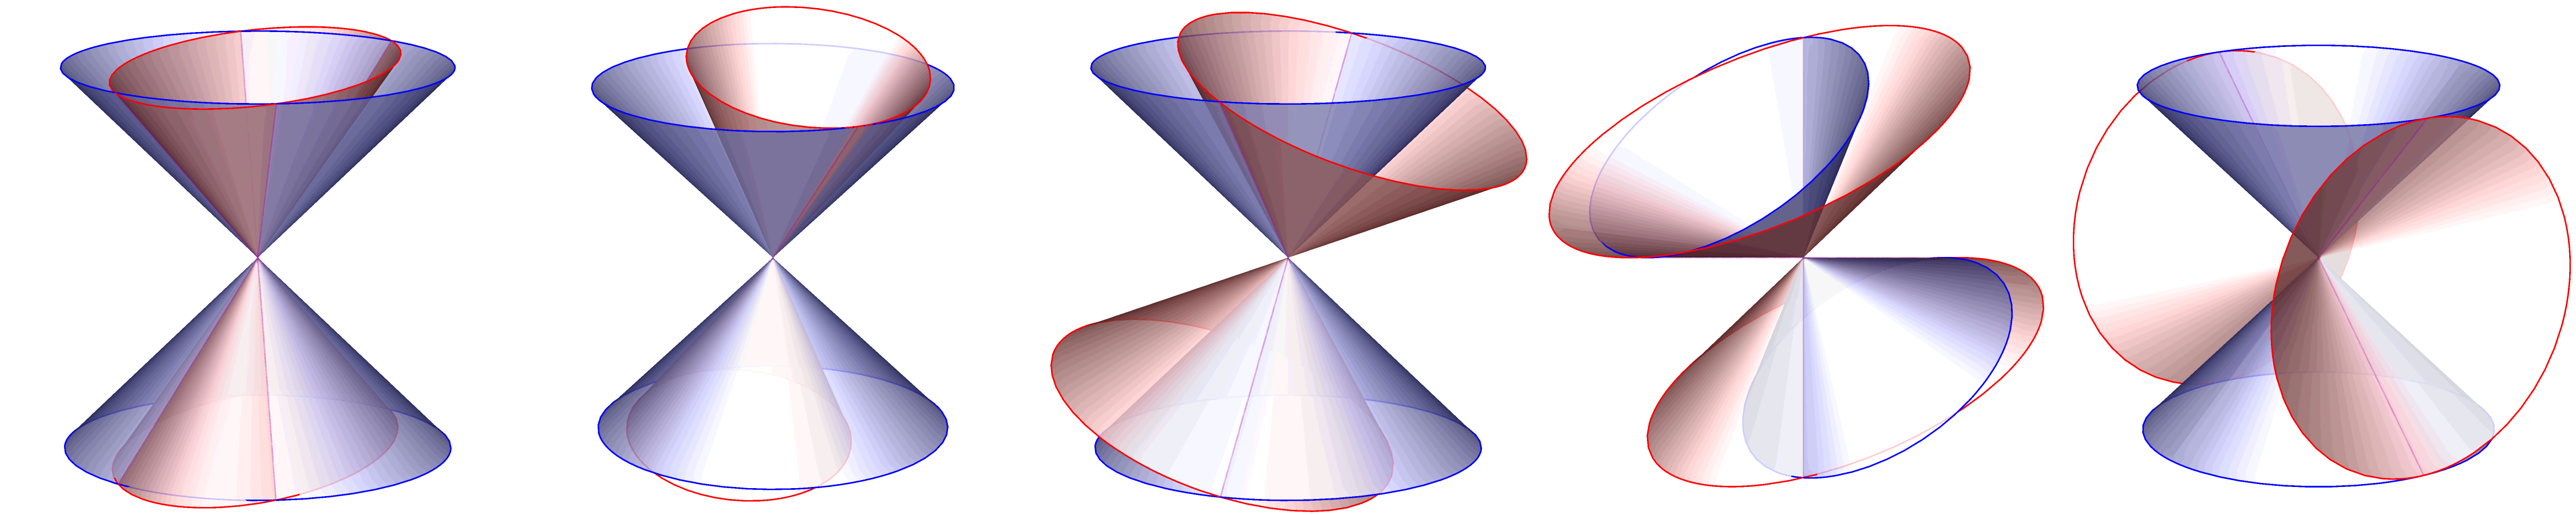
\includegraphics[width=\textwidth]{figures/test-figure}
  };
  \node[] at (0*28+14,0) {Type I};
  \node[] at (1*28+14,0) {Type IIa};
  \node[] at (2*28+14,0) {Type IIb};
  \node[] at (3*28+14,0) {Type III};
  \node[] at (4*28+14,0) {Type IV};
  \end{tikzpicture}\vspace{-0.6ex}
  
  \caption{\label{fig:classification}Allowed null cone configurations.}
\end{figure}

\begin{table}[H]
  \caption{\label{tab:classification}Allowed local metric configurations.}
  \vspace{-1ex}
  
  \noindent\centering{}\hspace{-3mm}
  \bgroup\renewcommand{\arraystretch}{1.5}
  \begin{tabular}{cccc} \hline\hline
    Type % & Segre char. 
    & $\diag(g)$ & $\diag(f)$ & $\diag(g^{-1}f)$ 
    \\ \hline
    \textbf{I} % & $[1111]$ 
    & $(-1,1,1,1)$ 
    & $(-\lambda_1,\lambda_2,\lambda_3,\lambda_4)$
    & $(\lambda_1,\lambda_2,\lambda_3,\lambda_4)$
    \\
    \textbf{IIa} % & $[211]$ 
    & $(\pm\!
    \begin{pmatrixc} 0&1\\[-0.2em]1&0\end{pmatrixc}\!,1,1 )$
    & $(\pm\!
    \begin{pmatrixc} 0&\lambda\\[-0.2em]\lambda & 1 \end{pmatrixc}\!,
    \lambda_2,\lambda_3)$
    & $(\begin{pmatrixc} \lambda&1\\[-0.2em]0 & \lambda \end{pmatrixc}\!,
    \lambda_2,\lambda_3)$
    \\[0.8em]
    \textbf{IIb} % & $[z\bar{z}11]$ 
    & $(\pm\!
    \begin{pmatrixc} 0 & 1 \\[-0.2em]1 & 0 \end{pmatrixc}\!,1,1)$ 
    & $(\pm\!
    \begin{pmatrixr}b & a \\[-0.2em] a & -b \end{pmatrixr}\!,
    \lambda_2,\lambda_3)$ 
    & $(
    \begin{pmatrixr}a & -b \\[-0.2em] b & a \end{pmatrixr}\!,
    \lambda_2,\lambda_3)$ 
    \\[0.8em]
    \textbf{III} % & $[31]$ 
    & $(\begin{pmatrixc} 0&0&1\\[-0.2em]
    0 & 1 & 0\\[-0.2em]
    1 & 0 & 0 \end{pmatrixc}\!,1)$
    & $(\begin{pmatrixc} 0&0&\lambda\\[-0.2em]
    0 & \lambda &1\\[-0.2em]
    \lambda & 1 & 0 \end{pmatrixc}\!,\lambda_2)$
    & $(\begin{pmatrixc} \lambda&1&0\\[-0.2em]
    0 & \lambda &1\\[-0.2em]
    0 & 0 & \lambda \end{pmatrixc}\!,\lambda_2)$
    \\
    \textbf{IV} % & $[(11)11]$ 
    & $(-1,1,1,1)$ 
    & $(\lambda,-\lambda,\lambda_2,\lambda_3)$
    & $(-\lambda,-\lambda,\lambda_2,\lambda_3)$
    \\ \hline\hline
  \end{tabular}
  \egroup
\end{table}
%%%%%%%%%%%%%%%%%%%%%%%%%%%%%%%%%%%%%%%%%%%%%%%%%%%%%%%%%%%%%%%%%%%%%%%%%%%%%
% chapters/chapter-3.tex
%%%%%%%%%%%%%%%%%%%%%%%%%%%%%%%%%%%%%%%%%%%%%%%%%%%%%%%%%%%%%%%%%%%%%%%%%%%%%

\chapter{Applications}
\label{chap:apps}


%%%%%%%%%%%%%%%%%%%%%%%%%%%%%%%%%%%%%%%%%%%%%%%%%%%%%%%%%%%%%%%%%%%%%%%%%%%%%
% chapters/summary.tex
%%%%%%%%%%%%%%%%%%%%%%%%%%%%%%%%%%%%%%%%%%%%%%%%%%%%%%%%%%%%%%%%%%%%%%%%%%%%%

\chapter{Summary and outlook}

The results of Paper \ref{art:A} are relevant for ...

%%%%%%%%%%%%%%%%%%%%%%%%%%%%%%%%%%%%%%%%%%%%%%%%%%%%%%%%%%%%%%%%%%%%%%%%%%%%%
% chapters/summary-swe.tex
%%%%%%%%%%%%%%%%%%%%%%%%%%%%%%%%%%%%%%%%%%%%%%%%%%%%%%%%%%%%%%%%%%%%%%%%%%%%%

\chapter*{Svensk sammanfattning}
\addcontentsline{toc}{chapter}{Svensk sammanfattning}

A short summary in Swedish should be be included if the thesis 
is written in a foreign language.


%----------------------------------------------------------------------------
% REFERENCES
%----------------------------------------------------------------------------

\cleardoublepage
\addtocounter{chapter}{1}
\renewcommand{\bibname}{References}
\renewcommand{\ThumbBoxColor}{red}

\newcommand{\RefsBox}{\ThumbBox{Refs}{0}}
\fancypagestyle{plain}
{
   \fancyhead[CE]{\RefsBox}
   \fancyhead[CO]{\RefsBox}
}
\fancyhead[CE]{\RefsBox}
\fancyhead[CO]{\RefsBox}

\bibliographystyle{biblio/JHEP}
\bibliography{biblio/lic-thesis}

%%%%%%%%%%%%%%%%%%%%%%%%%%%%%%%%%%%%%%%%%%%%%%%%%%%%%%%%%%%%%%%%%%%%%%%%%%%%%
% PAPERS
%%%%%%%%%%%%%%%%%%%%%%%%%%%%%%%%%%%%%%%%%%%%%%%%%%%%%%%%%%%%%%%%%%%%%%%%%%%%%

\label{lastPageOfPartI}
\cleardoublepage

\renewcommand{\RefsBox}{}

\fancypagestyle{plain}
{
    \fancyhf{}
    \fancyfoot[LE,RO]{\thepage}
    \renewcommand{\headrulewidth}{0pt}
    \renewcommand{\footrulewidth}{0pt}
}

\fancyhf{}
\fancyhead[LE,RO]{\thepage}

\newcommand{\paperSection}[6]{  % Arguments:
  \def\PaperID{#1}           % ID of the paper I, II, ...
  \def\PaperTitle{#2}        % Title that goes to the table of contents
  \def\PaperInfo{#3}         % Info that goes to the separation page
  \def\PaperFile{#4}         % Filename of the PDF in papers/ folder
  \def\PaperFolioX{#5}       % X position of our folio (page number)
  \def\PaperFolioY{#6}       % Y position of our folio (page number)
  \labelPaper{\PaperID}
  \addtocounter{chapter}{1}
  \pagestyle{plain}
  \phantomsection
  \addcontentsline{toc}{chapter}{\numberline{\hspace{-2mm}\PaperID}\PaperTitle}
  ~ % No text here (everything is in the overlay)
  \ThumbBoxLarge{Paper~\PaperID}{-5}
  \overlayPaperInfo{\PaperInfo}
  \cleardoublepage
}

\newcommand{\includePDF}[1]{
  \ifIncludePDFs
    \pagestyle{empty}
    \includepdf[pages={-}, noautoscale=true, #1,
      pagecommand={
        \noindent\ThumbBox{Paper~\PaperID}{-5}
        \overlayPaperFolio{\thepage}{\PaperFolioX}{\PaperFolioY}
      }]{papers/\PaperFile.pdf}
    \cleardoublepage
  \fi
}

\phantomsection
\addcontentsline{toc}{part}{Part II \;Papers}
\renewcommand{\ThumbBoxColor}{black}

%----------------------------------------------------------------------------
% Paper I
%----------------------------------------------------------------------------

\paperSection{I}
  {Paper title}
  {Authors,
    \emph{Paper title}, 
    [\href{https://arxiv.org/abs/1706.07806}{1706.07806}]}
  {1706-07806}{2}{\ifSpaper 8.7 \else 20 \fi}
\label{art:A} % PDF

\renewcommand{\PaperSubFolioFontSize}{10}
\setcounter{PaperSubFolio}{0}

\ifSpaper
  \includePDF{scale=0.96,offset=-2mm 0mm}
\else
  \includePDF{scale=1,offset=2mm 0mm}
\fi

%----------------------------------------------------------------------------
% Paper II
%----------------------------------------------------------------------------

\paperSection{II}
  {Paper title}
  {Authors, 
    \emph{Paper title}, 
    [\href{https://arxiv.org/abs/1708.07833}{1708.07833}]}
  {1708-07833}{2}{\ifSpaper 8.7 \else 20 \fi}
\label{art:B}

\renewcommand{\PaperSubFolioFontSize}{10}
\setcounter{PaperSubFolio}{0}

\ifSpaper
  \includePDF{scale=0.96,offset=-2mm 0mm}
\else
  \includePDF{scale=1,offset=2mm 0mm}
\fi

%----------------------------------------------------------------------------
% Paper III
%----------------------------------------------------------------------------

\paperSection{III}
  {Paper title}
  {Authors,
    \emph{Paper title}, 
    Phys.~Rev.~D96 (2017) no.~6, 064003, 
    doi:\href{http://doi.org/10.1103/PhysRevD.96.064003}
    {10.1103/PhysRevD.96.064003}, 
    [\href{https://arxiv.org/abs/1703.07787}{1703.07787}]}
  {1703-07787}{1}{\ifSpaper 19.1 \else 20.8 \fi}
\label{art:C}

\renewcommand{\PaperSubFolioFontSize}{9}
\setcounter{PaperSubFolio}{1}

\ifSpaper
  \includePDF{scale=0.87,offset=-2mm 0mm}
\else
  \includePDF{scale=0.98,offset=1mm 0mm}
\fi

%%%%%%%%%%%%%%%%%%%%%%%%%%%%%%%%%%%%%%%%%%%%%%%%%%%%%%%%%%%%%%%%%%%%%%%%%%%%%
% Show LAYOUT INFO (optional)
%%%%%%%%%%%%%%%%%%%%%%%%%%%%%%%%%%%%%%%%%%%%%%%%%%%%%%%%%%%%%%%%%%%%%%%%%%%%%

\pagestyle{empty}

\ifShowLayout
  \setcounter{chapter}{1}
  \phantomsection
  \renewcommand*{\FrameEdgeColor}{blue!40}
  \renewcommand*{\ShowSubGridColor}{gray!40}
  \renewcommand*{\ShowGridColor}{gray!70}
  \renewcommand*{\ShowFrameColor}{\color{red!40}}
  \renewcommand*{\ShowGridTextColor}{gray}
  % \renewcommand*{\ShowFramePicture}{}
  \AddToShipoutPictureBG{
     \ThumbBoxLarge{Paper~L}{0}
     \ThumbBox{Tab 5}{4}
     \ThumbBox{Tab 10}{9}
  }
  \noindent
  % \textsf{\textbf{Layout info}}\\[2mm]
  \setvaluestextsize{\footnotesize}
  \footnotesize
  \printinunitsof{mm}{\pagevalues}\\
  ~\verb| \marginparwidth| = 
  \printinunitsof{mm}\prntlen{\marginparwidth}
  ~\verb|   \TopOffset| = 
  \printinunitsof{mm}\prntlen{\TopOffset}\\
  ~\verb| \FontSize| = \FontSize
  \ifSpaper
     \setlayoutscale{0.45}
  \else
     \setlayoutscale{0.5}
  \fi
  \pagediagram
  \setvaluestextsize{\normalsize}
  \normalsize
\else
  ~
\fi

\end{document}
